\subsection{UC 6.1.1: File}
		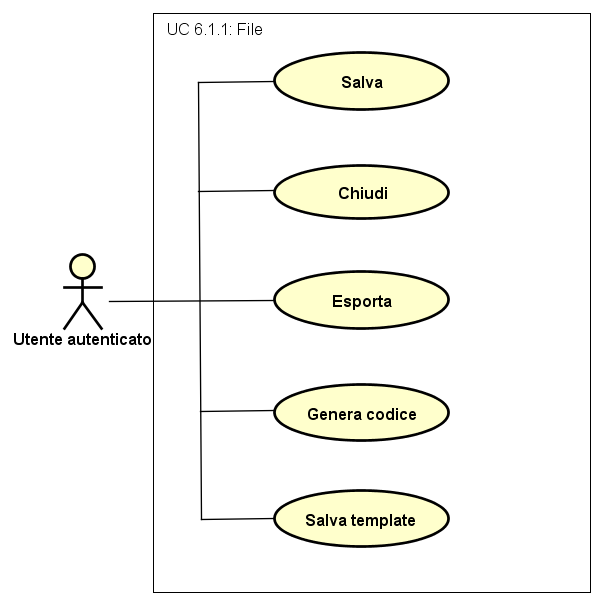
\includegraphics[scale=0.8]{../../Casi D'uso/UC 6.1.1.png}
\begin{itemize}
		\item \textbf{Attori coinvolti:} Utente autenticato. \\
		\item \textbf{Scopo e descrizione:} L'utente autenticato può accedere alle voci save, close, export e generates code appartenenti alla voce file del menù. \\
		\item \textbf{Precondizione:} L'applicazione offre all'utente la voce file nella barra dei menù. \\
		\item \textbf{Postcondizione:} L'applicazione, a seconda dell'operazione richiesta dall'utente, svolge le sue funzioni. \\
\end{itemize}